\chapter{Developer Documentation}
\label{dev}
\section{Overview}
\label{sec:overview}
\subsection{File structure}
\dirtree{%
    .1 /stack-prog-synth.
    .2 stackprogsynth.
    .3 data.
    .3 gui.
    .3 lang.
    .3 nn.
    .3 beamSearch.py.
    .3 constants.py.
    .3 utils.py.
    .2 tests.
    .3 data.
    .3 lang.
    .3 test\_utils.py.
    .2 environment.yml.
    .2 gen.py.
    .2 main.py.
    .2 train.py.
    .2 treelstm.pyi.
}

The tree above shows the file structure of the whole project. This is a joint work of a fellow student Xie Zongpu and me. 

\texttt{stack-prog-synth} is the project folder and \texttt{stackprogsynth} is the source folder, the following was written by me:
\begin{enumerate}
    \item \texttt{lang} folder, except \texttt{type.py}: for data generation, encoding, and program evaluation.
    \item \texttt{nn} folder, except \texttt{data.py}: for building the model and measuring the accuracy.
    \item \texttt{gui} folder and \texttt{main.py} file: for graphical user interface.
    \item \texttt{constants.py} file: storing constant parameters for synthetic data generation and network construction. 
\end{enumerate}

The figure below shows the dependencies of files on my part. \texttt{main.py} is in the root folder \texttt{stack-prog-synth} while all other paths are relative to the source folder which is \texttt{stackprogsynth}. The file \texttt{beamSearch.py} was written by my colleague, however, it is necessary to be included in the figure since this part serves as an important bond between different modules.
\begin{figure}[H]
    \centering
    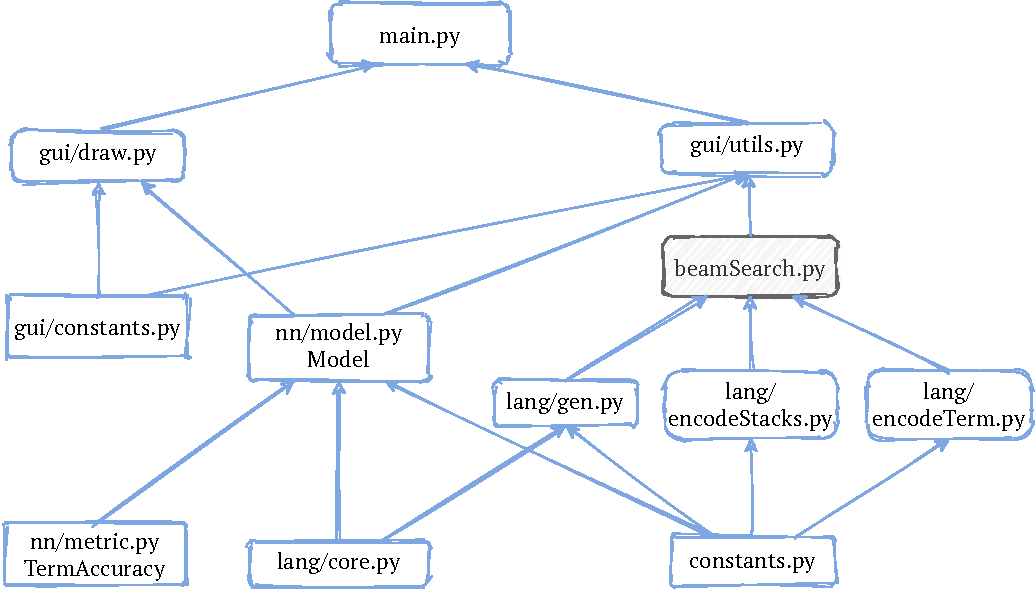
\includegraphics[width=1.0\textwidth]{dependencies.pdf}
    \caption{Dependencies of modules}
    \label{fig:dep}
\end{figure}
The next session will give a brief summary of each module and the following sections will explain the implementation of each part in detail.

\subsection{Software architecture}
Figure \ref{fig:uml} is the class diagram that covers most part of the project. It shows the connections between separate modules. 
\begin{figure}[H]
    \centering
    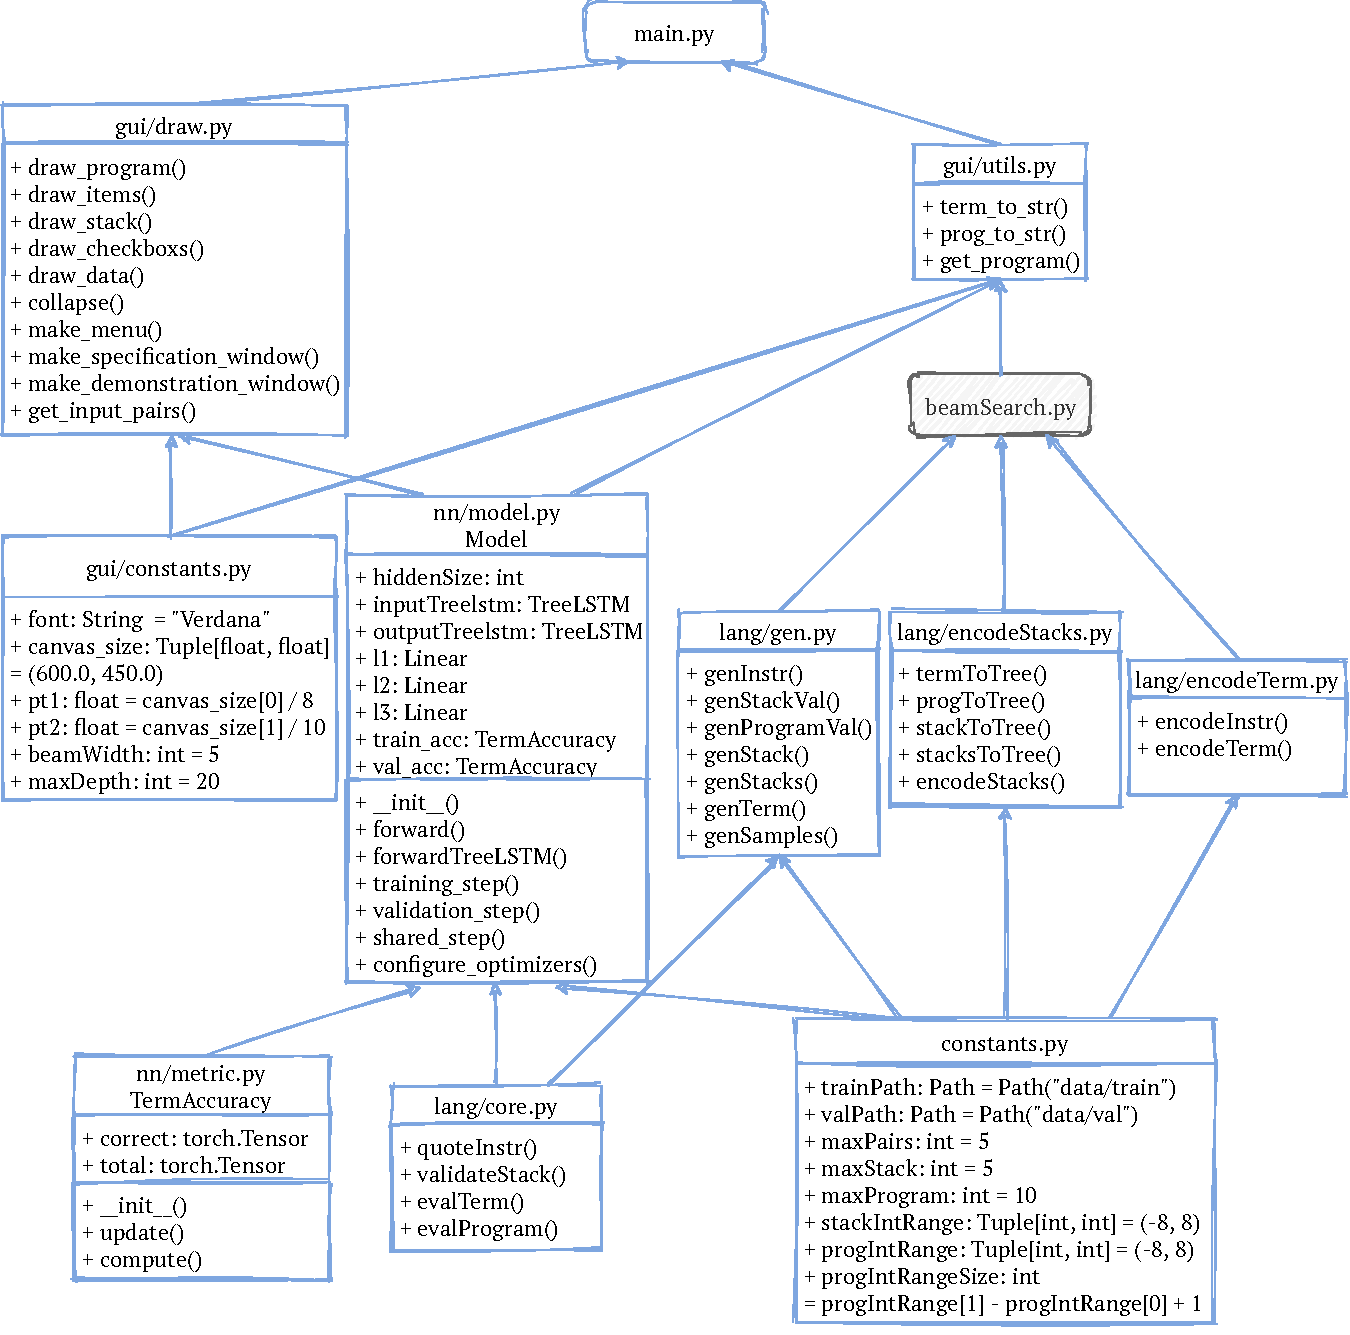
\includegraphics[width=1.05\textwidth]{UML.pdf}
     \caption[Connections between different modules; (function parameters and return types are omitted)]
    {\tabular[t]{@{}l@{}}Connections between different modules \\ (function parameters and return types are omitted)\endtabular}
    \label{fig:uml}
\end{figure}
To start with, the user can run \texttt{main.py} to start the program. It has the main function that uses PySimpleGUI \cite{psgui} to render windows and handle events. Coordinating with \texttt{draw.py} and \texttt{utils.py}, it is able to pass user input to the beam search algorithm and get the predicted result.

File \texttt{draw.py} offers functions for stack animations and layout design. In \texttt{utils.py}, \texttt{get\_program} will give trained model to \texttt{beamSearch} to obtain the prediction, and \texttt{prog\_to\_str} will convert the program to string so that it can be displayed in the window.  \texttt{constants.py} in \texttt{gui} folder has constant parameters for rendering the window and using the beam search algorithm.

\texttt{model.py} has the class \texttt{Model}. It inherits \texttt{LightningModule} from the PyTorch Lightning \cite{pytorch-ligntning} library. This custom class has methods to build the network, create Tree-LSTM and linear layer, and train the model. It also has instances of \texttt{TermAccuracy} to measure the performance of the prediction.

\texttt{gen.py} is used for synthetic data generation, this will be discussed in detail in Section \ref{sec:datagen}. Files \texttt{encodeStack.py} and \texttt{encodeTerm.py} are used to convert data structures to tree then encode them, so that the Tree-LSTM layer can be applied. Section \ref{sec:encoding} will talk more about this.

The file \texttt{core.py}, as the name suggests, contains the core of the language. It implements the stack-based concatenative languge, see details in Section \ref{sec:impdsl}. The evaluation functions \texttt{evalTerm} and \texttt{evalProgram} are used to get the target result from the input. \texttt{validateStack} checks the integer ranges in the stack and \texttt{quoteInstr} converts an instruction to a quotation.

In the root folder, \texttt{constants.py} defines constant arguments for data synthesis and layer creation. It contains integer ranges that are used by the encoding files for validation. And the stack size and program length are used by \texttt{gen.py} for generating stack values and programs.

\subsection{General workflow}
The following figure gives an overview of the whole project. The part inside the rectangle is the architecture of our neural network, and this will be discussed in Section \ref{sec:network}.

Generally speaking, we generate random input stacks and programs, by running the evaluation function \texttt{evalProgram} in \texttt{core.py}, we can get the corresponding output stacks. We then encode the input and output stacks and feed them into the Tree-LSTM neural network. Using supervised learning, we encoded the desired output program at the same time and compare it with the result that is given by the model. After this, the neural network will calculate the loss and the Adam optimizer \cite{adamW} will make mini-batch gradient descent and back-propagation \cite{BP}, repeat the training process until the model reaches a decent validation accuracy. 

When the model is prepared, we can use beam search on it to predict terms. Given input and output pairs, our trained model will give a probability for each term. The beam search algorithm then will rank the scores and find the most suitable fit as a solution.
\begin{figure}[H]
    \centering
    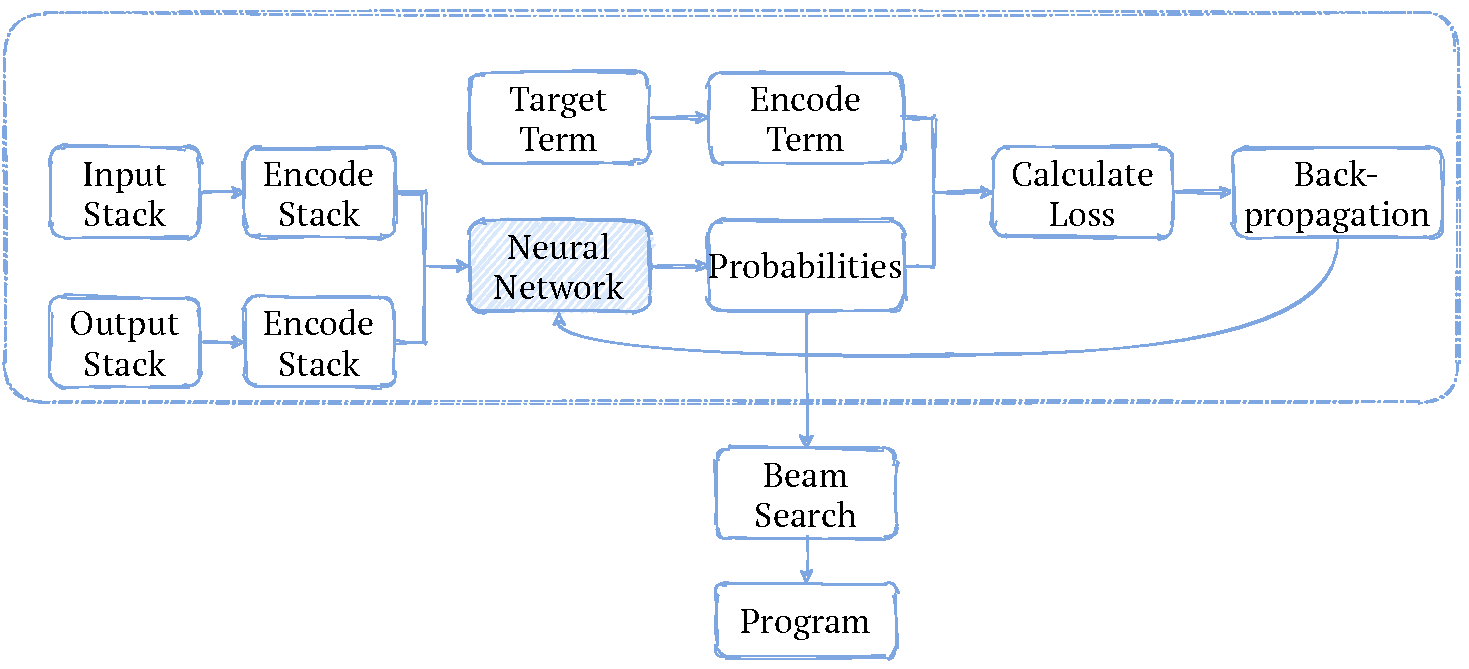
\includegraphics[width=0.85\textwidth]{workflow.pdf}
    \caption{Workflow}
    \label{fig:workflow}
\end{figure} 

\section{DSL in Implementation}
\label{sec:impdsl}
The following shows the UML for implementation of the stack-based concatenative language. 

\texttt{Instr}, \texttt{Val}, \texttt{Int} and \texttt{Quoted} are classes for the ADT constructor. \texttt{Term}, \texttt{Program}, \texttt{Instruction} and \texttt{Value} are type synonyms, with \texttt{Term} defined as \texttt{T.Union[Instr, Val]}, \texttt{Instruction} defined as \texttt{T.Union[
    Swap, Dup, Pop, Comp, Id, Quote, Apply, Dip, Add, Sub, Mul, Div, Mod
]} and \texttt{Value} defined as \texttt{T.Union[Quoted, Int]}.

Type \texttt{Union} in the typing module \cite{typing} was used to in the procedure. \texttt{Union[X, Y]} mean either X or Y. Similar to inheritance \cite{wiki:inheritance} in object-oriented programming \cite{wiki:oop}, it represents subtypes from base types. However, it is closed for extensions \cite{wiki:open-closed}.

\texttt{Program} is the type synonym of \texttt{Deque[Term]}. The abstract data type \texttt{Deque} gives back a new object instead of changing the original. This makes programs more efficient to manipulate persistently, meaning it allows access to any version, old or new, at any time \cite{driscoll1989making}. When using the beam search algorithm, we need to be able to append to one version of the structure in multiple ways so as to check different possible terms.

\begin{figure}[H]
    \centering
    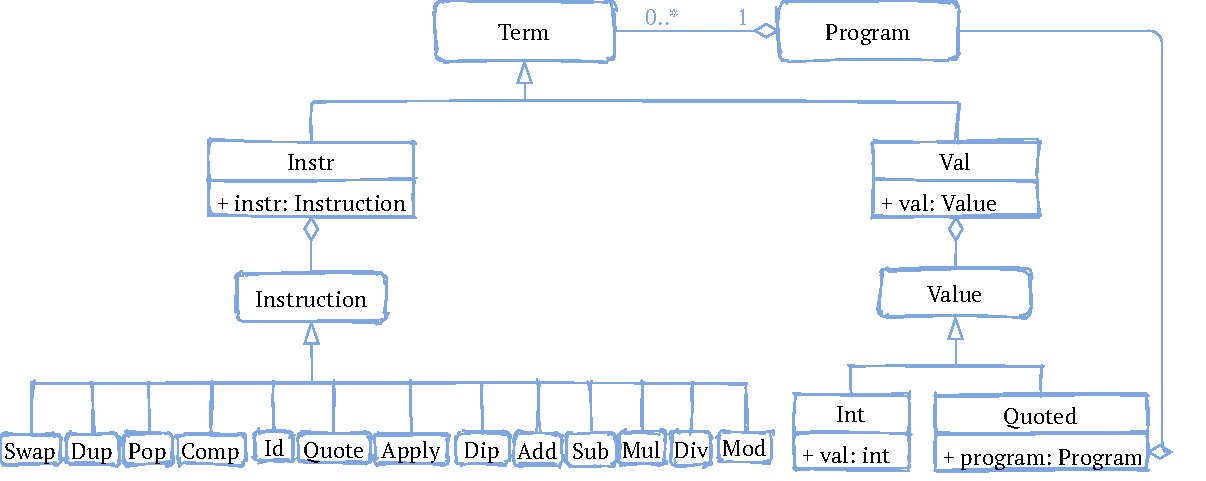
\includegraphics[width=\textwidth]{UML-Lang.pdf}
    \caption{Class diagram of the stack language AST}
    \label{fig:uml-lang}
\end{figure}

Section \ref{sec:lang} has a detailed description of each instruction and \texttt{evalTerm} implements the functionalities of each of them. Values are pushed to the stack. Integer operations \texttt{Add}, \texttt{Sub}, \texttt{Mul}, \texttt{Div} and \texttt{Mod} expect two integer values on the top of the stack. Some functions expect quoted programs on top of the stack and execute them in many different ways, effectively by dequoting, examples are \texttt{Apply} and \texttt{Dip}. The code below shows a small part of evaluating a term on a stack in \texttt{evalTerm} function.

\begin{listing}[H]
\begin{minted}{python}
        if isinstance(term.instr, Comp):
            fst, stack = stack.pop()
            snd, stack = stack.pop()
            if isinstance(fst, Quoted) and isinstance(snd, Quoted):
                return stack.push(Quoted(deque(snd.program + fst.program)))
            raise ValueError(fst, snd)
        if isinstance(term.instr, Id):
            return stack.push(Quoted(deque()))
        if isinstance(term.instr, Quote):
            value, stack = stack.pop()
            return stack.push(Quoted(deque([Val(value)])))
\end{minted}
\caption{Implementation of Comp, Id, and Quote}
\end{listing}

\section{Data Processing}
\label{sec:datagen}
\subsection{Synthetic data generation}
Synthetic data is artificial data generated to preserve privacy, testing systems, or creating training data for machine learning algorithms. 
Synthetic data generation is critical since it is an important factor in the quality of synthetic data \cite{synthdata}. 
If one does not have clean and well-prepared data, they may encounter garbage in, garbage out situations. Besides, the performance of a machine learning model is upper bounded by the quality of the data \cite{dataquality}. Therefore, generating enough amount of data with good quality is not only a prerequisite but also one of the requirements for a successful model training.

For our project, we need to generate stacks and programs separately. We treated a tuple of an input stack and a term and the resulting stack as one sample. Figure \ref{fig:gen} illustrates the functions we wrote for synthesizing data and the relationship between them. And here follows how we generated samples in detail. 

\begin{wrapfigure}{l}{0.5\textwidth}
    \centering
    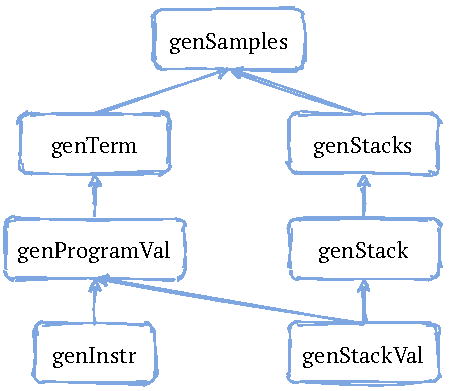
\includegraphics[width=0.5\textwidth]{gen.pdf}
    \caption{Functions for data generation}
    \label{fig:gen}
\end{wrapfigure}

For programs, we have \texttt{genProgramVal} which creates random integer values in a predetermined range and uses \texttt{genInstr} to generate instructions. The \texttt{genTerm} function gets a random stack, returns a tuple of a generated term, and a tuple of new stacks. It will prune away invalid stacks or redundant programs. 

For stacks, \texttt{genStack} uses \texttt{genStackVal} to get random integer values within a certain bound, for the sake of simplicity, we now only allow input stacks to have integers. \texttt{genStacks} returns a tuple that contains \texttt{maxPairs} of stacks, and each stack has a length that equals to \texttt{maxStack}. Finally, \texttt{genSamples} (see Listing \ref{fun:genSamples}) uses \texttt{genTerm}  and \texttt{genStacks} to return a list of samples. \texttt{genTerm} checks the type of the new term and the elements in the new stacks. \texttt{genSamples} managed to avoid repetition of stacks in the resulting list.

\begin{listing}[H]
\begin{minted}{python}
def genSamples(
    rng: Random = Random(),
) -> T.List[T.Tuple[T.Tuple[Stack[Value], ...], T.Tuple[Stack[Value], ...], Term]]:
    samples: T.List[T.Tuple[T.Tuple[Stack[Value], ...], Term]] = []
    currStacks = genStacks(rng)
    inStacks = currStacks
    progNum = rng.randint(1, maxProgram)
    result = {currStacks}

    for _ in range(progNum):
        newTerm, newStacks = genTerm(inStacks, rng)
        if newStacks not in result:
            result.add(newStacks)
            samples.append((currStacks, newTerm))
            currStacks = newStacks
    return [(inp, currStacks, newTerm) for (inp, newTerm) in samples]
\end{minted}
\caption{genSamples function}
\label{fun:genSamples}
\end{listing}

It is important to note in advance that integers are infinite, we have to set bound to them in order to do the encoding before passing them to the neural network. All the predetermined ranges are written in \texttt{constants.py} file. We set the range of integers in the program from -8 to 8, since small numbers are more frequent and a program with small numbers can manipulate big numbers. The file also defines the maximum size of a stack and the maximum allowed number of input-output pairs in a stack. These settings will not restrict our program to a large extent since integers can always get bigger numbers by adding or multiplying and stacks can expand. 
\subsection{Abstract syntax tree embedding}
\label{sec:ast}
By having quotations in our stacks, they can have programs as first-class functions, which makes them not linear structures anymore. As a result, we need to look for neural networks that are suitable for tree-structured inputs instead of using the conventional recurrent neural network which is for linear data. We decided to use Tree-structured Long Short-Term Memory \cite{tree-lstm} networks to deal with non-linearity. Tree-LSTM is a generalization of LSTM which works on tree-structured inputs. We used a Python library \texttt{pytorch-tree-lstm} \cite{pytorch-tree-lstm}. It is an implementation of the child sum Tree-LSTM model \cite{tree-lstm}, and it supports vectorized tree evaluation and batching.
\begin{figure}[H]
    \centering
    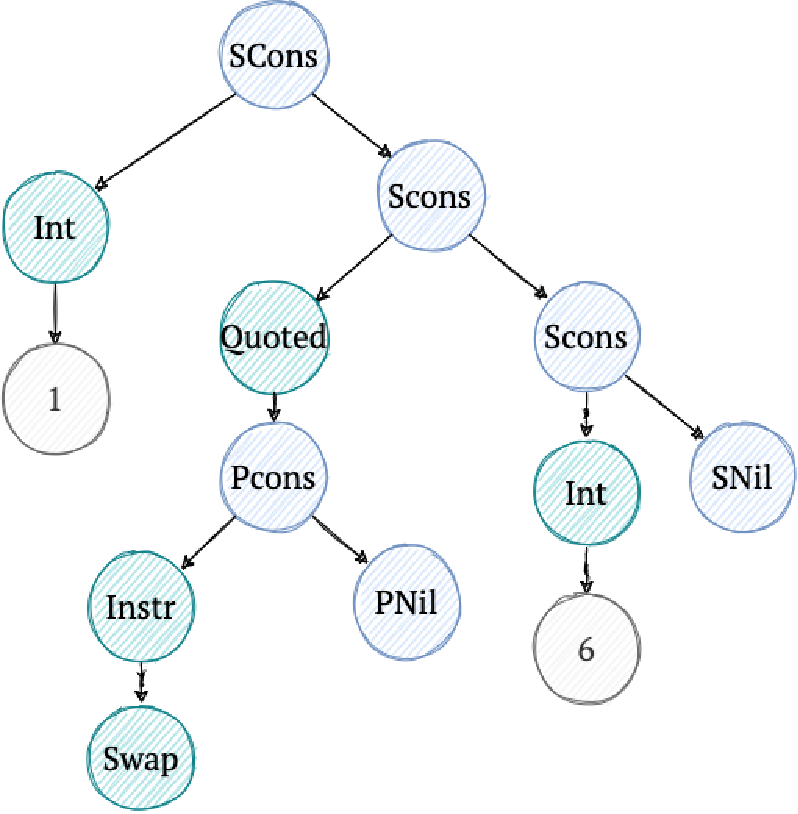
\includegraphics[width=0.5\textwidth]{tree.pdf}
    \caption{Abstract syntax tree}
    \label{fig:tree}
\end{figure}
First, we need to convert stacks to trees. As the example shown in Figure \ref{fig:tree}, by having constructors like SCons, SNil, PNil, Quoted (they are stored in \texttt{labelClasses}, see Listing \ref{labels}), we can turn the stack $<Int(1), Quoted([Instr(Swap)]), Int(6)>$ to a tree. Then, with the help of the library, we are able to convert each node to a tensor so that it can be given to the Tree-LSTM structure.  

\begin{listing}[H]
\begin{minted}{python}
labelClasses: T.List[T.Union[str, int]] = (
    [
        constr.__name__
        for constr in T.get_args(Term) + T.get_args(Value) + T.get_args(Instruction)
    ]
    + ["PCons", "PNil", "SCons", "SNil", "TCons", "TNil"]
    + [i for i in range(stackIntRange[0], stackIntRange[1] + 1)]
)
\end{minted}
\caption{labelClasses}
\label{labels}
\end{listing}

\subsection{Encoding}
\label{sec:encoding}
From Figure \ref{fig:workflow} we can deduce that it is necessary to encode stacks and target terms before training. 

\begin{wrapfigure}{r}{0.5\textwidth}
    \centering
    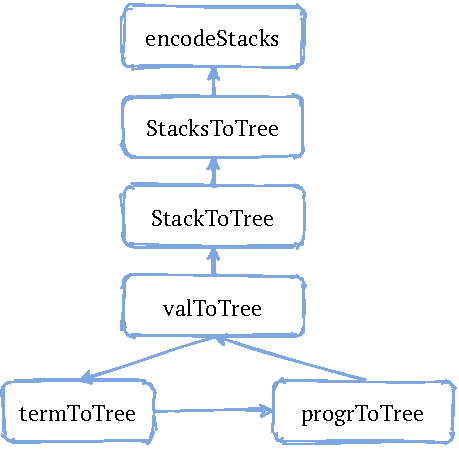
\includegraphics[width=0.5\textwidth]{encode.pdf}
    \caption{Functions for encoding stacks}
    \label{fig:encode}
\end{wrapfigure}

Figure \ref{fig:encode} exhibits the functions written for encoding stacks, the names are self-explanatory. In order to apply the Tree-LSTM layer on the stacks, it is important to first convert them to trees before encoding. As we saw in Figure \ref{fig:syntax}, programs comprise terms and terms consist of values, and quoted programs can be values. Hence, the functions \texttt{termToTree}, \texttt{progToTree} and \texttt{valToTree} are mutually recursive, it is like normal recursion where a function uses itself, they instead use each other. Mutual recursion is very common in functional programming.

The listings \ref{lst:encodeInstr} and \ref{lst:encodeTerm} are code for encoding instructions and terms. For instructions encoding, we return one plus the corresponding index of the given instruction. Since the 0th place is reserved for non-instruction types.

\begin{listing}[H]
\begin{minted}{python}
def encodeInstr(instr: Instruction) -> int:
    return T.get_args(Instruction).index(instr.__class__) + 1
\end{minted}
\caption{Function for encoding an instruction}
\label{lst:encodeInstr}
\end{listing}

\begin{listing}[H]
\begin{minted}{python}
class EncodedTerm:
    termLabel: int
    instrLabel: int
    integer: int
\end{minted}
\caption{EncodedTerm class}
\label{code:encodedTerm}
\end{listing}

\texttt{encodeTerm} returns a tuple of type \texttt{EncodedTerm}, it is a class that we created to store the encoding result, as the Listing \ref{code:encodedTerm} shows. It has three fields:
\begin{itemize}
    \item \texttt{termLabel}: Indicating the type of the new term,  0 for instructions, 1 for quotations, and 2 for integers.
    \item \texttt{instrLabel}: Specifying the type of the instruction, 0 for integers.
    \item \texttt{integer}: Representing the integer value, 0 for non-integer types and 1 to predetermined \texttt{progIntRangeSize} for integers. 
\end{itemize}

In \texttt{encodeTerm}, the \texttt{isinstance} function returns True if the specified object is of the specified type, otherwise False. We have two validations here:
\begin{itemize}
    \item Whether the quotation has only a single instruction.
    \item Whether the integer value within the predefined range.
\end{itemize}

A \texttt{ValueError} will be raised if the validation fails, otherwise, it returns an \texttt{EncodedTerm} instance.
\begin{listing}[H]
\begin{minted}{python}
def encodeTerm(term: Term) -> EncodedTerm:
    if isinstance(term, Instr):
        return EncodedTerm(0, encodeInstr(term.instr), 0)
    if isinstance(term, Val):
        if isinstance(term.val, Quoted):
            prog = term.val.program.left()
            if isinstance(prog, Instr):
                return EncodedTerm(1, encodeInstr(prog.instr), 0)
            raise ValueError(prog)
        if isinstance(term.val, Int):
            intVal = term.val.val
            if intVal < progIntRange[0] or intVal > progIntRange[1]:
                raise ValueError("Integer value out of range.")
            return EncodedTerm(2, 0, intVal - progIntRange[0] + 1)
\end{minted}
\caption{Function for encoding a term}
\label{lst:encodeTerm}
\end{listing}


\section{Network Construction}
\label{sec:network}
In this section, we will first give a holistic view of the network structure, then explain the implementation of network building, layer creating, and model training in detail. And hyper-parameters are listed in the end.

\subsection{Network architecture and classes}
Figure \ref{fig:nn} shows the architecture of our neural network. We mainly used the \texttt{PyTroch} \cite{pytorch} library to build the neural net. The input of it is input and output stacks of a single program. Following the steps described in Section \ref{sec:ast}, we encode the stacks and feed them into Tree-LSTM networks. 

In the hidden linear layers, the model learns and improves by evaluating the input and comparing it with the target output. We wrote a custom class to score the output and this will be discussed in Section \ref{sec:termacc}.  

\begin{figure}[H]
    \centering
    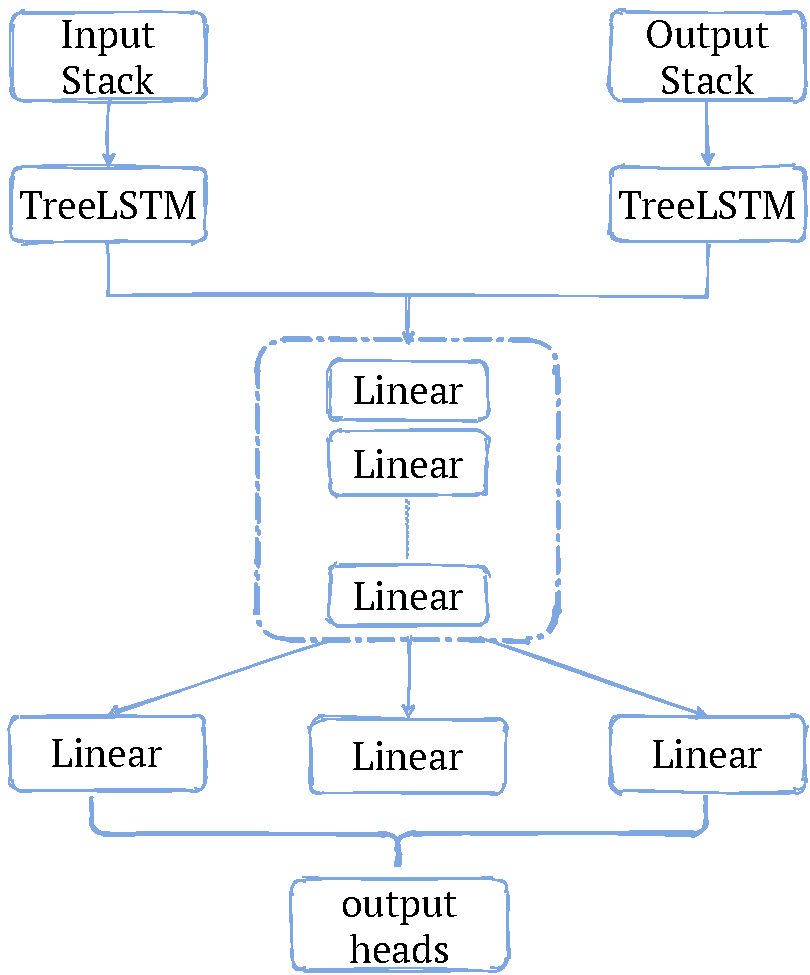
\includegraphics[width=0.4\textwidth]{nn.pdf}
    \caption{Network architecture}
    \label{fig:nn}
\end{figure}

In this stage, the \texttt{pytorch-tree-lstm} \cite{pytorch-tree-lstm} library helps the model increase efficiency in evaluating. Usually, efficient batching of tree data is complicated. It needs to evaluate all of a node's children before it can evaluate the node itself. To minimize the performance impact of this issue, the library breaks the node evaluation process into steps. In this way, each step it evaluates all nodes for which all child nodes have been previously evaluated. This allows the user to evaluate multiple nodes with each torch operation, increasing computation speeds by an order of magnitude over recursive approaches.

Take Figure \ref{fig:tree} for example, on the first step of the tree calculation, the library can evaluate nodes 1, Swap, 6, PNil and SNil in parallel as they are all leaves of the tree, i.e. none of them has any child nodes. At the second step, it will evaluate node Int, Instr, as their child nodes were evaluated previously. Finally, it evaluates node 0, which depends on nodes 1 and 2. By doing this, the library can reduce a 13-node computation to six steps. As the dataset gets larger and trees get bigger with more leaf nodes, the user can experience larger performance gains.

The network's output heads finally produce 3 vectors, corresponding to the three fields of \texttt{EncodeTerms} explained in Section \ref{sec:encoding} 

\begin{figure}[H]
    \centering
    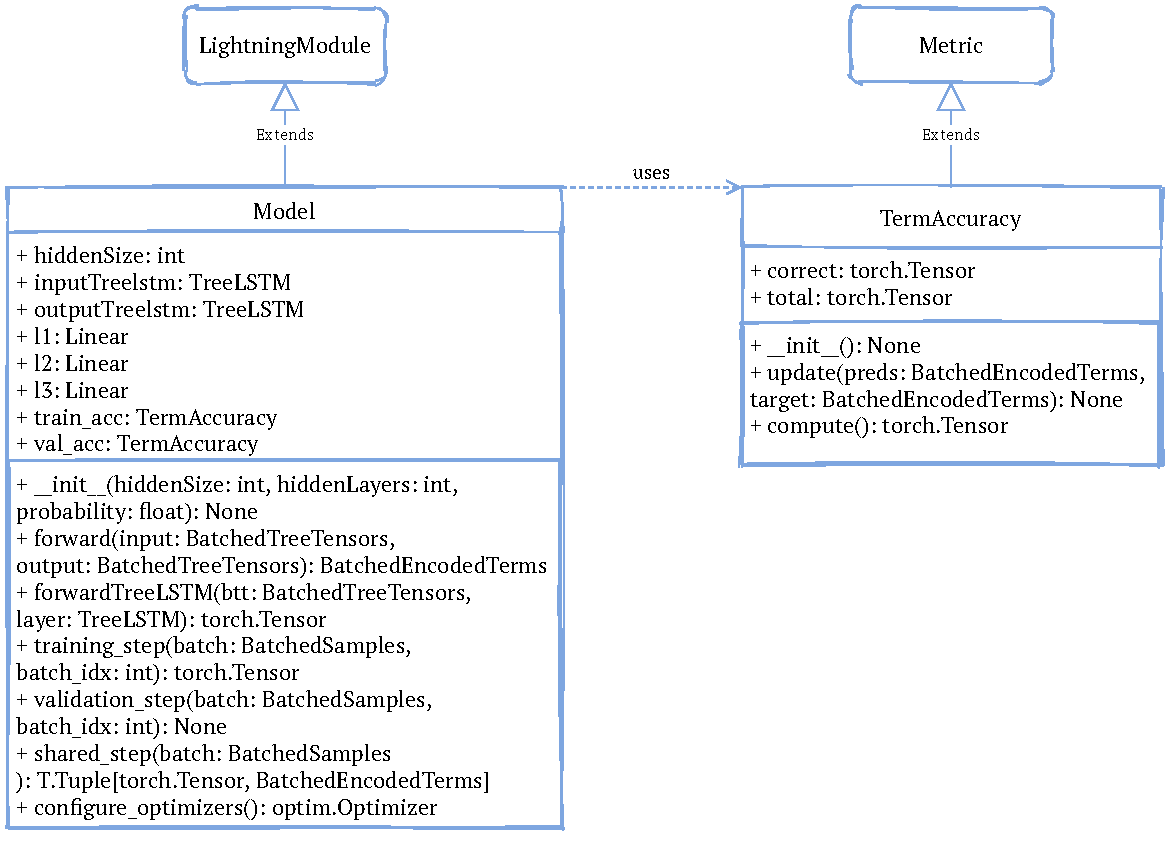
\includegraphics[width=1.02\textwidth]{classes.pdf}
    \caption{Model class and TermAccuracy class}
    \label{fig:classes}
\end{figure}

The image above is a class diagram for \texttt{Model} and \texttt{TermAccuracy}. They extends classes \texttt{LightningModule} and \texttt{Metric}, both of them are from the PyTorch Lightning \cite{pytorch-ligntning} library. Section \ref{sec:buildnn} to Section \ref{sec:train} goes through all the functions in the \texttt{Model} class, and Section \ref{sec:termacc} talks the class \texttt{TermAccuracy} in detail.

\subsection{Building the network}
\label{sec:buildnn}
Having seen the structure of the whole network, we are now going to see the implementation of it. 

Listing \ref{lst:cons} shows the constructor of the model. We have the number of nodes in each middle layer (\texttt{hiddenSize}), the number of hidden layers (\texttt{hiddenLayers}).

\begin{listing}[H]
\begin{minted}{python}
def __init__(self, hiddenSize: int, hiddenLayers: int):
    super().__init__()
    self.save_hyperparameters()
    self.hiddenSize = hiddenSize
    # Input layers
    self.inputTreelstm = TreeLSTM(len(labelClasses), hiddenSize)
    self.outputTreelstm = TreeLSTM(len(labelClasses), hiddenSize)
    # Hidden layers
    self.hidden = nn.ModuleList()
    for i in range(hiddenLayers):
        middle = nn.Linear(2 * hiddenSize, 2 * hiddenSize)
        self.hidden.append(middle)
    # Output layers
    self.l1 = nn.Linear(2 * hiddenSize, 1 + len(T.get_args(Value)))
    self.l2 = nn.Linear(2 * hiddenSize, 1 + len(T.get_args(Instruction)))
    self.l3 = nn.Linear(2 * hiddenSize, 1 + progIntRangeSize)
    
    self.train_acc = TermAccuracy()
    self.val_acc = TermAccuracy()
\end{minted}
\caption{Model constructor}
\label{lst:cons}
\end{listing}
We first create two Tree-LSTM layers for input and output stacks, the size of each input sample is the number of all the constructors for the abstract syntax tree and the number of features of the output of both layers is the hidden size. We concatenated two Tree-LSTM layers together before going through linear layers. Hence, the input and output size of middle layers are twofold of \texttt{hiddenSize}. Three output layers correspond to the output heads elaborated in \ref{sec:network}. 

\subsection{Applying layers}
Here follows how the input is processed through the network. We have \texttt{forwardTreeLSTM} and \texttt{forward} to do this job.

\texttt{forwardTreeLSTM} is used to apply Tree-LSTM layers to inputs. Four tensors \texttt{features}, \texttt{adjacency\_list}, \texttt{node\_order}, and \texttt{edge\_order} store the encoded tree structure and features.
Since the calculation of Tree-LSTM goes bottom up, we select the root nodes as the final result. The \texttt{unbatch\_tree\_tensor} is from the \texttt{pytorch-tree-lstm} library \cite{pytorch-tree-lstm}, it is used to unbatch the batched samples into a list. And we used \texttt{torch.unsqueeze} to create a new outer dimension to concatenate the samples.
\begin{listing}[H]
\begin{minted}{python}
def forwardTreeLSTM(self, btt: BatchedTreeTensors, layer: TreeLSTM) -> torch.Tensor:
    # Applying the layer.
    result, _ = layer(
        btt["features"].float(),
        btt["node_order"],
        btt["adjacency_list"],
        btt["edge_order"],
    )
    # Acquiring the calculated features of the root node for each sample.
    result = [
        torch.unsqueeze(sample[0], 0)
        for sample in unbatch_tree_tensor(result, btt["tree_sizes"])
    ]
    return torch.cat(result)
\end{minted}
\caption{Tree-LSTM layers}
\end{listing}

In \texttt{forward} ,the comment \mintinline{python}{type: ignore[override]} is used to silence the type checker on this line caused by incompatible overrides. Here we first concatenate two Tree-LSTM layers together, then use a for loop to add enough number of middle layers to the module list in the constructor and use \texttt{relu} activation function on each of them. And finally, return a tuple of three output heads. The class \texttt{BatchedEncodedTerms} has the same fields as \texttt{EncodedTerm} in Listing \ref{code:encodedTerm}, but the type of them is \texttt{torch.Tensor} instead of \texttt{int}.

\begin{listing}[H]
\begin{minted}{python}
def forward(  # type: ignore[override]
    self, input: BatchedTreeTensors, output: BatchedTreeTensors
) -> BatchedEncodedTerms:
    input1 = self.forwardTreeLSTM(input, self.inputTreelstm)
    input2 = self.forwardTreeLSTM(output, self.outputTreelstm)
    middle = torch.cat((input1, input2), 1)
    for i in range(len(self.hidden)):
        middle = self.hidden[i](middle)
        middle = nn.functional.layer_norm(middle, [self.hiddenSize * 2])
        middle = F.relu(middle)
    o1 = self.l1(middle)
    o2 = self.l2(middle)
    o3 = self.l3(middle)
    return BatchedEncodedTerms(o1, o2, o3)
\end{minted}
\caption{Network layers}
\end{listing}

\subsection{Training and improving model}
\label{sec:train}
\texttt{shared\_step} uses cross-entropy to measure the loss of three output tensors from the forward layer. It returns a tuple of the sum of the loss and the predicted result, and this step is necessary for both training and validation stages. \texttt{training\_step} and \texttt{validation\_step} are basically the same except that they used different datasets. 

\begin{listing}[H]
\begin{minted}{python}
def shared_step(
    self, batch: BatchedSamples
) -> T.Tuple[torch.Tensor, BatchedEncodedTerms]:
    predicted = self.forward(batch.input, batch.output)
    loss1 = nn.functional.cross_entropy(predicted.termLabel, batch.target.termLabel)
    loss2 = nn.functional.cross_entropy(
        predicted.instrLabel, batch.target.instrLabel
    )
    loss3 = nn.functional.cross_entropy(predicted.integer, batch.target.integer)
    return (loss1 + loss2 + loss3, predicted)
\end{minted}
\caption{The common step}
\end{listing}

\begin{listing}[H]
\begin{minted}{python}
def training_step(
    self, batch: BatchedSamples, batch_idx: int
) -> torch.Tensor:  # type: ignore[override]
    loss, predicted = self.shared_step(batch)
    accuracy = self.train_acc(predicted, batch.target)
    self.log("train_loss", loss)
    self.log("train_acc", accuracy, prog_bar=True)
    return loss

def validation_step(
    self, batch: BatchedSamples, batch_idx: int
) -> None:  # type: ignore[override]
    loss, predicted = self.shared_step(batch)
    accuracy = self.val_acc(predicted, batch.target)
    self.log("val_loss", loss, prog_bar=True)
    self.log("val_acc", accuracy, prog_bar=True)
\end{minted}
\caption{Training and validating}
\end{listing}

We used AdamW \cite{adamW} as the optimizer. It has an adaptive learning rate, with default parameter starting from 0.001. This enables it to solve problem of slower convergence in the late stage of training.
\begin{listing}[H]
\begin{minted}{python}
    def configure_optimizers(self) -> optim.Optimizer:
        return optim.AdamW(self.parameters())
\end{minted}
\caption{AdamW optimizer}
\end{listing}

\subsection{Measuring the accuracy}
\label{sec:termacc}
Evaluating the machine learning algorithm is an essential part of any project. Accuracy is one metric to measure how often the algorithm classifies a data point correctly. It is the ratio of the number of correct predictions to the total number of input samples.
\[Accuracy=\frac{Number\ of\ correct\ predictions}{Total\ number\ of\ predictions}\]

The accuracy of our model is measured by the sum of the three tensors generated by the output heads. We wrote our custom class for measuring it. \texttt{argmax} can find the class with the largest predicted probability.
\begin{listing}[H]
\begin{minted}{python}
class TermAccuracy(Metric):
    correct: torch.Tensor
    total: torch.Tensor
    def __init__(self) -> None:
        super().__init__()
        self.add_state("correct", default=torch.tensor(0), dist_reduce_fx="sum")
        self.add_state("total", default=torch.tensor(0), dist_reduce_fx="sum")

    def update(self, preds: BatchedEncodedTerms, target: BatchedEncodedTerms) -> None:
        t1 = torch.argmax(preds.termLabel, dim=1) == target.termLabel
        t2 = torch.argmax(preds.instrLabel, dim=1) == target.instrLabel
        t3 = torch.argmax(preds.integer, dim=1) == target.integer
        combined = torch.sum(t1 & t2 & t3)
        self.correct += combined
        self.total += torch.tensor(target.termLabel.numel())

    def compute(self) -> torch.Tensor:
        return self.correct.float() / self.total
\end{minted}
\caption{Custom Accuracy class}
\end{listing}


\subsection{Hyper-parameters and loss functions}
Hyper-parameters are parameters of the structure of the neural network, they can control the process of learning. We train our models with the following parameters:
\begin{itemize}
    \item Batch size: 32
    \item Middle layers: 5
    \item Hidden nodes: 1000
    \item Optimizer: AdamW
    \item Loss function: cross entropy
    \item Activation function: relu
\end{itemize}


\section{Testing}
\label{sec:test}
An application without testing is not trustworthy. Automated tests can be very useful for killing bugs in application development. It also keeps validating the code while adding new code or refactoring old code. 

There is a great number of functions that need to be tested in the project, and each function may need multiple test cases. Putting all the test cases into one \texttt{tests.py} file might not be a maintainable and scalable way. Therefore, we created a \texttt{tests} package in the root folder, and split tests into two folders \texttt{data} and \texttt{lang} to test files in the corresponding \texttt{data} and \texttt{lang} folder in the project. They also represent two main testings in this project. Pytest \cite{pytest} is for unit testing in \texttt{data} folder and hypothesis test \cite{hytest} is used for property testing in \texttt{lang} folder.


\subsection{Unit tests}
Python has built-in \texttt{unittest} module. It provides a solid base on which to build the test suite, but it has a few shortcomings. A number of third-party testing frameworks attempt to address some of the issues with \texttt{unittest}, and pytest \cite{pytestbook} has proven to be one of the most popular. It is a mature and full-featured testing framework, from small tests to large-scale functional tests for applications and libraries alike.

\dirtree{%
    .1 /data.
    .2 test\_deque.py.
    .2 test\_llist.py.
    .2 test\_stack.py.
    .2 test\_tree.py.
}

The structure above shows the files in \texttt{data} folder. With the powerful pytest library, we tested four main data structures: \texttt{deque}, \texttt{llist}, \texttt{stack}, and \texttt{tree}. For each data structure, we tested their main methods and the important functions related to them.

In \texttt{data/test\_deque.py}, we have the tests cases for the methods of double-ended queue data structure. Here are two examples, they test the \texttt{appendleft} method and the \texttt{pop} method of deque.
\begin{listing}[H]
\begin{minted}{python}
@given(st.lists(st.integers()), st.integers())
def test_deque_appendleft(xs: T.List[int], x: int) -> None:
    assert deque(xs).appendleft(x) == deque([x] + xs)

@given(st.lists(st.integers()).filter(lambda x: x))
def test_deque_pop(xs: T.List[int]) -> None:
    assert deque(xs).pop() == (deque(xs[:-1]), xs[-1])
\end{minted}
\caption{Part of Deque testing}
\end{listing}

\subsection{Property tests}
Property-based testing has become quite famous in the functional world. It relies on properties which means that it checks that a function, program, or whatever system under test abides by a property. Most of the time, properties do not have to go into too many details about the output. They just have to check for useful characteristics that must be seen in the output. 

Here is the content in the \texttt{lang} folder. For each function in \texttt{core.py}, \texttt{encodeStacks.py} and \texttt{encodeTerm.py} file, we gave one to three test cases.

\dirtree{%
    .1 /lang.
    .2 test\_core.py.
    .2 test\_encodeStacks.py.
    .2 test\_encodeTerm.py.
}

The following are some examples in the \texttt{test\_encodeStacks.py} file. For function \texttt{valueToTree}, we tested two types of the value - \texttt{Int} and \texttt{Quoted} separately. The same logic applies to \texttt{termToTree} as well, we tested two subtypes of the term, \texttt{Instr} and \texttt{Val}.
\begin{listing}[H]
\begin{minted}{python}
def test_valueToTree_Int() -> None:
    assert valueToTree(Int(3)) == Tree("Int", [Tree(3, [])])

def test_valueToTree_Quoted() -> None:
    assert valueToTree(Quoted(deque([Instr(Add())]))) == Tree(
        "Quoted", [Tree("PCons", [Tree("Instr", [Tree("Add", [])]), Tree("PNil", [])])]
    )
\end{minted}
\caption{Test valueToTree}
\end{listing}

\begin{listing}[H]
\begin{minted}{python}
def test_termToTree_Val() -> None:
    assert termToTree(Val(Int(8))) == Tree("Val", [Tree("Int", [Tree(8, [])])])

def test_termToTree_Instr() -> None:
    assert termToTree(Instr(Dup())) == Tree("Instr", [Tree("Dup", [])])
\end{minted}
\caption{Test termToTree}
\end{listing}

For the function \texttt{encodeStacks}, the one-hot encoded result is tested. The \texttt{stack1} and \texttt{stack2} are predefined. For the return value, we check whether each row contains only one 1 and everything else is 0.
\begin{listing}[H]
\begin{minted}{python}
def test_encodeStacks() -> None:
    features = encodeStacks((stack1, stack2))["features"]
    for row in features:
        num = numel(row)
        cnt = bincount(row.int())
        assert cnt[0] == num - 1
        assert cnt[1] == 1
\end{minted}
\caption{Test encodeStacks}
\end{listing}

For \texttt{progToTree}, \texttt{stackToTree} and \texttt{stacksToTree} in \texttt{encodeStacks.py} and \texttt{encodeInstr}, \texttt{encodeTerm} in \texttt{encodeTerm.py}, we calculate the desired result manually, and compare them with the function output. The following shows tests in \texttt{test\_encodeTerm.py} file.
\begin{listing}[H]
\begin{minted}{python}
def test_encodeInstr() -> None:
    assert encodeInstr(Swap()) == 1

def test_encodeTerm() -> None:
    assert encodeTerm(Val(Int(3))) == EncodedTerm(2, 0, 12)
\end{minted}
\caption{Test encodeTerm.py file}
\end{listing}

In \texttt{test\_core.py} file, three test cases are given for each of \texttt{quoteInstr}, \texttt{validateStack}, and \texttt{evalProgram} function. And to test \texttt{evalTerm} function, we wrote test cases for each instruction.

\subsection{Testing results}
There are by far 60 tests altogether. We tested all the major functions, but we can always add more test cases for the same function for the sake of safety. The command to run all the tests in the \texttt{tests} folder is: \texttt{python -m pytest}. You will see the following results.
{\small
\begin{verbatim}
================================= test session starts ==================================
platform darwin -- Python 3.8.6, pytest-6.2.2, py-1.10.0, pluggy-0.13.1
rootdir: /Users/su/Desktop/stack-prog-synth
plugins: hypothesis-6.2.0
collected 60 items                                                                         
tests/test_utils.py .                                                           [  1%]
tests/data/test_deque.py ...........                                            [ 20%]
tests/data/test_llist.py .                                                      [ 21%]
tests/data/test_stack.py .......                                                [ 33%]
tests/data/test_tree.py ..                                                      [ 36%]
tests/lang/test_core.py ......................                                  [ 73%]
tests/lang/test_encodeStacks.py ........                                        [ 86%]
tests/lang/test_encodeTerm.py ..                                                [ 90%]
tests/lang/test_type.py ......                                                  [100%]

================================== 60 passed in 5.96s ==================================
\end{verbatim}
}